% !TeX program = xelatex
\documentclass[12pt,a4paper]{article}
\usepackage{fontspec}
\setmainfont{Times New Roman}
\usepackage[english,russian]{babel}
\usepackage{amsmath,amssymb,mathrsfs,cancel}
\usepackage[margin=22mm]{geometry}
\usepackage{graphicx,float}
\usepackage[unicode,hidelinks]{hyperref}
\DeclareMathOperator{\grad}{grad}
\DeclareMathOperator{\Div}{div}
\newcommand{\Rey}{\mathrm{Re}}
\setlength{\emergencystretch}{3em}
\sloppy
\interfootnotelinepenalty=10000
\newcommand{\topic}[1]{\par\medskip\noindent\textbf{#1}\par\nobreak\smallskip}
\renewcommand{\thefootnote}{\arabic{footnote})}
\begin{document}
\section*{Вопрос 11}
Модель двухфазного течения в пренебрежении капиллярной разностью давлений (модель Маскета — Мереса). Опрокидывание волны повышения насыщенности в задаче об одномерном течении (в задаче Бакли — Леверетта). Условия на скачках насыщенности.

\medskip
\noindent\textbf{Источник:} Г. И. Баренблатт, В. М. Ентов, В. М. Рыжик. \textit{Теория нестационарной фильтрации жидкости и газа}. Москва: Недра, 1972. Глава VI, § 2, с. 155--164.
\par\bigskip
\section*{Глава VI. Фильтрация неоднородных жидкостей}
\subsection*{§ 2. Вытеснение несмешивающихся жидкостей. Задача Баклея--Леверетта}
% Источник: Barenblatt-et-al-1972.djvu; печатная страница: 155; страница файла: 157
Извлечение нефти из пласта в большинстве случаев происходит путем вытеснения ее водой или газом. Общая схема такого процесса изображена на рис. \ref{q11:fig-VI-6}. Вода либо поступает в нефтенасыщенную часть пласта, перемещаясь из водонасыщенных зон того же пласта (краевая зона), либо искусственно закачивается в пласт через специальные нагнетательные скважины. Таким же вытесняющим агентом может быть газ, находящийся в пласте или специально нагнетаемый. Нефть извлекается через эксплуатационные скважины, причем в ряде случаев вместе с нефтью извлекается и вода или газ, прорвавшиеся к эксплуатационным скважинам. Хотя обычно природный газ отбирается из пласта за счет его расширения при снижении давления,
\renewcommand{\thefigure}{VI.\arabic{figure}}\setcounter{figure}{5}
\begin{figure}[H]\centering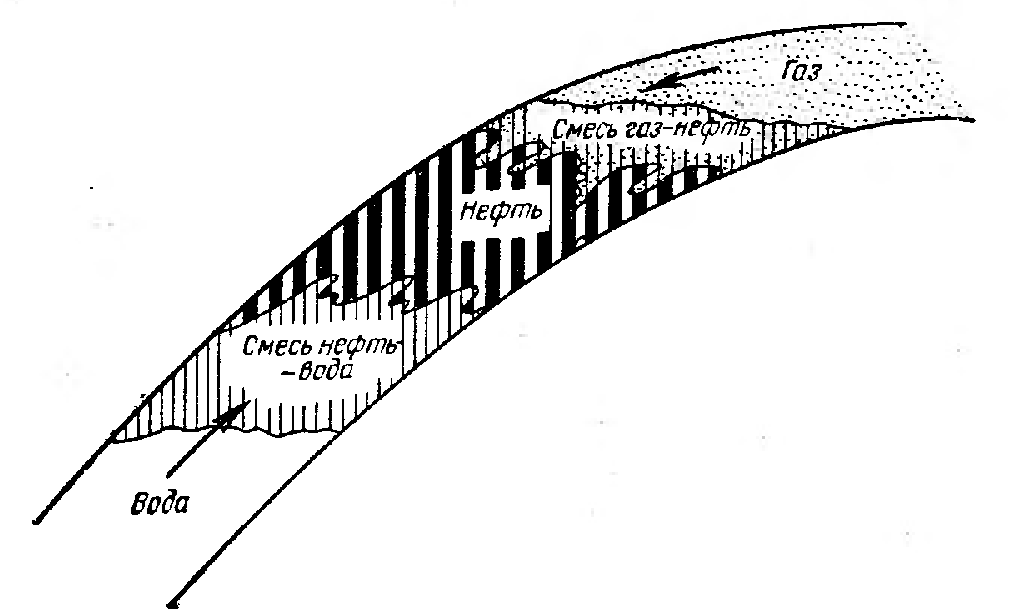
\includegraphics[width=.8\linewidth]{figures/fig-VI-6.png}\caption{}\label{q11:fig-VI-6}\end{figure}
% Источник: Barenblatt-et-al-1972.djvu; печатная страница: 156; страница файла: 158
в некоторых случаях и газовые пласты работают на режиме вытеснения газа водой, насыщающей внешние области того же пласта. Для анализа эффективности вытеснения нефти или газа несмешивающейся с ней жидкостью необходимо знать, как изменяется распределение насыщенности в пласте. В связи с этим вытеснение несмешивающихся жидкостей должно рассматриваться как процесс двухфазной фильтрации.

Выведем систему уравнений двухфазной фильтрации в однородной пористой среде без фазовых переходов. При записи закона фильтрации будем предполагать, что в любой точке каждая из фаз находится целиком лишь в одном из двух крайних состояний: а) связном и подвижном и б) несвязном и поэтому неподвижном. В соответствии со сказанным в предыдущем параграфе, в областях медленного термодинамически равновесного течения для тех жидкостей, которые можно считать связными, можно ввести в расчет зависящие только от насыщенности относительные проницаемости $f_i(s)$ и капиллярное давление $p_c(s)$.

Кроме того, не касаясь гистерезисных явлений, будем рассматривать только однонаправленные процессы, которые наиболее интересны для приложений.

В результате сделанных предположений закон фильтрации можно записать в виде:
\begin{equation}\bar u_i=-\frac{k}{\mu_i}f_i(s)\grad p_i\qquad(i=1,2).\tag{VI.2.1}\label{q11:eq-VI-2-1}\end{equation}
В равновесном однонаправленном течении разность давлений в фазах равна капиллярному давлению, определяемому формулами (VI.1.3) или (VI.1.4):
\begin{equation}p_2-p_1=p_c(s)=\alpha\sqrt{\frac{m}{k}}\cos\Theta J(s).\tag{VI.2.2}\label{q11:eq-VI-2-2}\end{equation}
Для определенности будем индекс 1 относить к более смачивающей фазе, насыщенность которой равна $s$. В задачах совместной фильтрации нефти или газа и воды более смачивающей фазой обычно является вытесняющая вода.

Для получения замкнутой системы уравнений необходимо записать уравнения сохранения массы для обеих фаз. Выделим в фильтрационном потоке некоторый объем $T$. Масса первой фазы в нем равна $\int_Tm\rho_1\,d\tau$ ($d\tau$ --- элемент объема $T$). Приток первой фазы за время $dt$ через поверхность $S$, ограничивающую объем $T$, составит $-dt\int_S\rho_1\bar u_1\bar n\,d\sigma$ ($\bar n$ --- вектор нормали к поверхности $S$, $d\sigma$ --- элемент поверхности $S$). Полагая, что в объеме $T$ не содержится источников массы, имеем
% В фразе о массе первой фазы в оригинале пропущен множитель s; сохранено.
\begin{equation}\frac{d}{dt}\int_Tm\rho_1s\,d\tau-\int_S\rho_1\bar u_1\bar n\,d\sigma=0,\tag{VI.2.3}\label{q11:eq-VI-2-3}\end{equation}
% Знак минус перед поверхностным интегралом напечатан в оригинале.
% Источник: Barenblatt-et-al-1972.djvu; печатная страница: 157; страница файла: 159
откуда, преобразуя поверхностный интеграл в объемный и учитывая, что объем $T$ произволен, а границы его неподвижны, получим окончательно
\begin{equation}\frac{\partial}{\partial t}(m\rho_1s)+\Div(\rho_1\bar u_1)=0.\tag{VI.2.4}\label{q11:eq-VI-2-4}\end{equation}
Аналогично выводится уравнение сохранения массы для второй фазы:
\begin{equation}\frac{\partial}{\partial t}[m\rho_2(1-s)]-\Div(\rho_2\bar u_2)=0.\tag{VI.2.5}\label{q11:eq-VI-2-5}\end{equation}
% В (VI.2.5) в оригинале минус перед div; сохранено.
Таким образом, мы получаем замкнутую систему уравнений для $p_1$ и $s$, поскольку $\rho_1$ и $\rho_2$ являются функциями давлений $p_1$ и $p_2$, а изменение пористости в однородном пласте зависит только от изменения среднего давления $\bar p=p_1s+p_2(1-s)$ (ср. гл. II), а не давления компонентов.

Если вытесняемая и вытесняющая фазы --- слабосжимаемые капельные жидкости, влиянием сжимаемости на распределение насыщенности можно пренебречь. Действительно, характерное время нестационарного перераспределения давления за счет сжимаемости имеет порядок $t_1=L^2/\varkappa$, где $\varkappa$ --- коэффициент пьезопроводности, $L$ --- характерный размер. Характерное время вытеснения --- порядка $t_2=L/u$, где $u$ --- средняя скорость фильтрации. Обычно скорость фильтрации --- около $10^{-3}$ см/сек, $L\approx10^4\div10^5$ см, а $\varkappa\approx10^4$ см$^2$/сек. Поэтому $t_1/t_2\approx10^{-2}$, откуда видно, что нестационарные процессы упругого перераспределения давления заканчиваются в начале хода вытеснения.

Если жидкости и пористую среду можно считать несжимаемыми, имеем вместо \eqref{q11:eq-VI-2-4} и (IV.2.5)
\begin{equation}m\frac{\partial s}{\partial t}+\Div\bar u_1=0,\qquad m\frac{\partial s}{\partial t}-\Div\bar u_2=0.\tag{VI.2.6}\label{q11:eq-VI-2-6}\end{equation}
% В отсылке оригинала напечатано IV.2.5; сохранено.
Решение системы уравнений \eqref{q11:eq-VI-2-1}, \eqref{q11:eq-VI-2-2}, \eqref{q11:eq-VI-2-6} для двух- или трехмерных случаев весьма сложно. Для анализа общих свойств поля насыщенности при вытеснении применим асимптотический подход, основанный на малости некоторых безразмерных параметров, входящих в условия задачи (см. работу Г. И. Баренблатта [26]).

В систему уравнений и граничные условия входят следующие размерные определяющие параметры: $\Delta p$ --- перепад давления между скважинами или галереями; $L$ --- характерный размер области течения; коэффициенты $k/\mu_1$ и $k/\mu_2$, а также $p_c^0=\alpha\sqrt{m/k}\cos\Theta$. Перейдем в уравнениях \eqref{q11:eq-VI-2-1}, \eqref{q11:eq-VI-2-2}, \eqref{q11:eq-VI-2-6} к безразмерным переменным:
\[\begin{gathered}
\frac{p_i}{\Delta p}=P_i;\quad\bar U_i=\frac{\bar u_i}{u_0};\quad\left(\bar u_0=\frac{k\Delta p}{\mu_1L}\right);\quad X=\frac{x}{L};\\
Y=\frac{y}{L};\quad Z=\frac{z}{L};\quad\tau=\frac{u_0t}{L}=\frac{k\Delta p}{\mu_1L^2}t;\quad\varepsilon=\frac{p_c^0}{\Delta p}.
\end{gathered}\]
% Источник: Barenblatt-et-al-1972.djvu; печатная страница: 158; страница файла: 160
Это приводит к системе уравнений
\begin{equation}\begin{gathered}
\bar U_1=-f_1(s)\grad P_2+\varepsilon f_1(s)J(s)\grad s;\\
\bar U_2=-\mu_0f_2(s)\grad P_2,\quad\mu_0=\mu_1/\mu_2
\end{gathered}\tag{VI.2.7}\label{q11:eq-VI-2-7}\end{equation}
% В первой строке (VI.2.7) в оригинале J(s) без штриха; сохранено.
(оператор $\grad$ выполняется здесь в переменных $X,Y,Z$):
\begin{equation}\begin{gathered}
m\frac{\partial s}{\partial\tau}+\frac{\partial U_{1X}}{\partial X}+\frac{\partial U_{1Y}}{\partial Y}+\frac{\partial U_{1Z}}{\partial Z}=0;\\
m\frac{\partial s}{\partial\tau}-\frac{\partial U_{2X}}{\partial X}-\frac{\partial U_{2Y}}{\partial Y}-\frac{\partial U_{2Z}}{\partial Z}=0.
\end{gathered}\tag{VI.2.8}\label{q11:eq-VI-2-8}\end{equation}
Уравнения \eqref{q11:eq-VI-2-7} записаны через $P_2$, так как только вытесняемая жидкость остается непрерывной во всей области течения, а вытесняющая может в целых областях, куда еще не дошел фронт вытеснения, находиться в виде отдельных капель.

Параметр $\varepsilon=p_c^0/\Delta p$ мал в большинстве интересных для приложений задач, так отмечалось в § 1. Поэтому член $\bar U_c=\varepsilon f_1(s)J'(s)\grad s$ может быть существен лишь в узких областях, где велик градиент насыщенности. Самый факт существования таких областей будет установлен позже, пока же отметим, что их протяженность должна быть мала по сравнению с основной внешней областью именно потому, что в них велик $|\grad s|$, а $s$ --- ограниченная величина. Это позволяет применить для анализа системы \eqref{q11:eq-VI-2-7}, \eqref{q11:eq-VI-2-8} метод асимптотического сращивания [36а], который заключается в использовании разных масштабов при рассмотрении движения в основной области и в узких зонах резкого изменения насыщенности. Подобно этому течение в пограничном слое вязкой жидкости вблизи стенок имеет иной пространственный масштаб, нежели внешнее течение.

Разделим область фильтрации на внешнюю зону, где $U_c$ --- малая величина, и узкую внутреннюю зону или зоны, где вследствие больших значений $|\grad s|$ членом $U_c$ пренебречь нельзя.

Малость параметра $\varepsilon$ приводит к естественной попытке исследовать течение во внешней зоне, разлагая искомое решение в степенной ряд по этому параметру (внешнее разложение). Первый член внешнего разложения мы получим, полагая $\varepsilon=0$. Исследование структуры внутренней зоны (внутреннее разложение) будет рассмотрено в следующем параграфе.

Общие свойства внешнего разложения рассмотрим вначале на примере одномерной задачи, решение которой получается в замкнутом виде.

В одномерном случае (плоском, радиальном или сферическом)
% Источник: Barenblatt-et-al-1972.djvu; печатная страница: 159; страница файла: 161
уравнения \eqref{q11:eq-VI-2-8} с учетом \eqref{q11:eq-VI-2-7} при $\varepsilon=0$ запишем, возвращаясь к размерным переменным, в виде:
\begin{equation}\begin{gathered}
m\frac{\partial s}{\partial t}-\frac{k}{\mu_1}\frac{1}{x^{\nu-1}}\frac{\partial}{\partial x}\left(x^{\nu-1}f_1(s)\frac{\partial p}{\partial x}\right)=0;\\
m\frac{\partial s}{\partial t}+\frac{k}{\mu_2}\frac{1}{x^{\nu-1}}\frac{\partial}{\partial x}\left(x^{\nu-1}f_2(s)\frac{\partial p}{\partial x}\right)=0\qquad(p_1=p_2=p)
\end{gathered}\tag{VI.2.9}\label{q11:eq-VI-2-9}\end{equation}
($\nu=1,2,3$ соответственно для линейного, радиального или сферического течения).

Вычитая второе уравнение \eqref{q11:eq-VI-2-9} из первого и интегрируя, получим
\begin{equation}[f_1(s)+\mu_0f_2(s)]\frac{\partial p}{\partial x}=\frac{C(t)}{x^{\nu-1}}\qquad\left(\mu_0=\frac{\mu_1}{\mu_2}\right).\tag{VI.2.10}\label{q11:eq-VI-2-10}\end{equation}
Это равенство выражает постоянство суммарного расхода вдоль трубки тока в силу несжимаемости жидкостей. Определяя $\partial p/\partial x$ из \eqref{q11:eq-VI-2-10} и подставляя в любое из уравнений \eqref{q11:eq-VI-2-9}, получим одно уравнение для $s$:
\begin{equation}\frac{\partial s}{\partial t}+\frac{q(t)}{m}\frac{F'(s)}{x^{\nu-1}}\frac{\partial s}{\partial x}=0,\tag{VI.2.11}\label{q11:eq-VI-2-11}\end{equation}
где $q(t)=-\dfrac{k}{\mu_1}C(t)$ --- суммарный расход жидкости через трубку тока, а
\[F(s)=\frac{f_1(s)}{f_1(s)+\mu_0f_2(s)}.\]
Функция $F(s)$ равна отношению скорости фильтрации (или расхода) вытесняющей фазы к суммарной скорости фильтрации (или к суммарному расходу). Функцию $F(s)$ принято называть функцией распределения фаз.

Введем новые независимые переменные: $Q=\int_{t_0}^t\dfrac{q(t)}{m}\,dt$, $W=\dfrac{x^\nu}{\nu}$.

Величину $W$ можно рассматривать как объем трубки тока между сечениями $x_0$ и $x$ (в частности, при $\nu=1$ и $q(t)=\mathrm{const}$ переменная $Q$ пропорциональна времени, а $W=x$). Тогда вместо \eqref{q11:eq-VI-2-11} имеем
\begin{equation}\frac{\partial s}{\partial Q}+F'(s)\frac{\partial s}{\partial W}=0.\tag{VI.2.12}\label{q11:eq-VI-2-12}\end{equation}
Этому уравнению в частных производных первого порядка соответствует следующая система характеристических уравнений:
\begin{equation}\frac{dQ}{1}=\frac{dW}{F'(s)}=\frac{ds}{0}.\tag{VI.2.13}\label{q11:eq-VI-2-13}\end{equation}
Общее решение системы \eqref{q11:eq-VI-2-13} представляется в виде:
\begin{equation}\begin{gathered}s=C_1;\\W=QF'(s)+C_2.\end{gathered}\tag{VI.2.14}\label{q11:eq-VI-2-14}\end{equation}
% Источник: Barenblatt-et-al-1972.djvu; печатная страница: 160; страница файла: 162
Таким образом, вдоль характеристик уравнения \eqref{q11:eq-VI-2-12} $s=\mathrm{const}$, и в плоскости $(W,Q)$ характеристики представляют собой прямые линии. Физически это означает, что каждое значение насыщенности $s$ распространяется со скоростью $dW/dQ$, пропорциональной $F'(s)$. В случае движения плоскими волнами $\nu=1$, а $\dfrac{dW}{dQ}$ есть истинная скорость распространения данного значения насыщенности.

На основании равенств \eqref{q11:eq-VI-2-14} общее решение уравнения \eqref{q11:eq-VI-2-12} можно формально записать в виде:
\begin{equation}W=QF'(s)+W_0(s),\tag{VI.2.15}\label{q11:eq-VI-2-15}\end{equation}
где функция $W_0(s)$ соответствует начальному распределению насыщенности (при $Q=0$, т. е. $t=t_0$).

На скважинах (или галереях), через которые нагнетается вытесняющая жидкость, должны быть заданы условия, определяющие состав нагнетаемой жидкости. Если нагнетается одна (вытесняющая) жидкость, то такое условие записывается в виде:
\begin{equation}u_2=-\frac{k}{\mu_2}f_2(s)\frac{\partial p}{\partial x}=0.\tag{VI.2.16}\label{q11:eq-VI-2-16}\end{equation}
Поскольку $\partial p/\partial x\ne0$, так как не равен нулю суммарный расход, то из (VI.2.5) следует $f_2(s)=0$, $s\le s_{**}$. Пусть в начальный момент везде в пласте насыщенность вытесняющей фазы ниже, чем $s_{**}$ ($s_{**}$ --- насыщенность, при которой вытесняемая фаза становится неподвижной). Это условие выполняется почти во всех задачах, имеющих физический смысл. Тогда при $t>0$ на границе будет выполняться условие
\begin{equation}s=s_{**}.\tag{VI.2.17}\label{q11:eq-VI-2-17}\end{equation}
% В предшествующей фразе отсылка VI.2.5 и знак ≤ напечатаны в оригинале.
Действительно, если предположить, что в некоторой точке границы $s>s_{**}$, то в силу непрерывности насыщенности вблизи этой точки границы должна существовать целая область конечных размеров, в которой $s>s_{**}$ и $u_2=0$. В силу уравнения неразрывности для вытесняемой фазы \eqref{q11:eq-VI-2-6} отсюда следует $\partial s/\partial t=0$. Это противоречит условию $s\le s_{**}$ при $t=0$. Если же задано отношение расходов двух фаз на поверхности нагнетания $\lambda$, то условие на границе имеет вид:
\begin{equation}\mu_0\frac{f_2(s)}{f_1(s)}=\lambda,\tag{VI.2.18}\label{q11:eq-VI-2-18}\end{equation}
откуда также определяется насыщенность на границе, поскольку относительные проницаемости $f_1(s)$ и $f_2(s)$ известны.

Вернемся к анализу общего вида решения \eqref{q11:eq-VI-2-15}.

На рис. \ref{q11:fig-VI-7}, \textit{а, б} изображены типичные кривые $F(s)$ и $F'(s)$. Функция $F'(s)$ имеет максимум в некоторой точке $s_m$. Поэтому в соответствии с формулой \eqref{q11:eq-VI-2-15} два разных значения насыщенности могут иметь одинаковую скорость распространения. В связи с этим получаемая по формуле \eqref{q11:eq-VI-2-15} зависимость насыщенности от $W$
% Источник: Barenblatt-et-al-1972.djvu; печатная страница: 161; страница файла: 163
может стать неоднозначной --- большие значения «обгоняют» меньшие, как это показано на рис. \ref{q11:fig-VI-8}.

Неоднозначность формального решения, получаемого из \eqref{q11:eq-VI-2-15}, означает, что непрерывных решений задачи о вытеснении при заданном начальном условии не существует. Чтобы получить решение, имеющее физический смысл, необходимо вводить разрывы (скачки) насыщенности, т. е. поверхности, на которых значение насыщенности меняется скачком. Такие скачки могут существовать и в начальных условиях.
\begin{figure}[H]\centering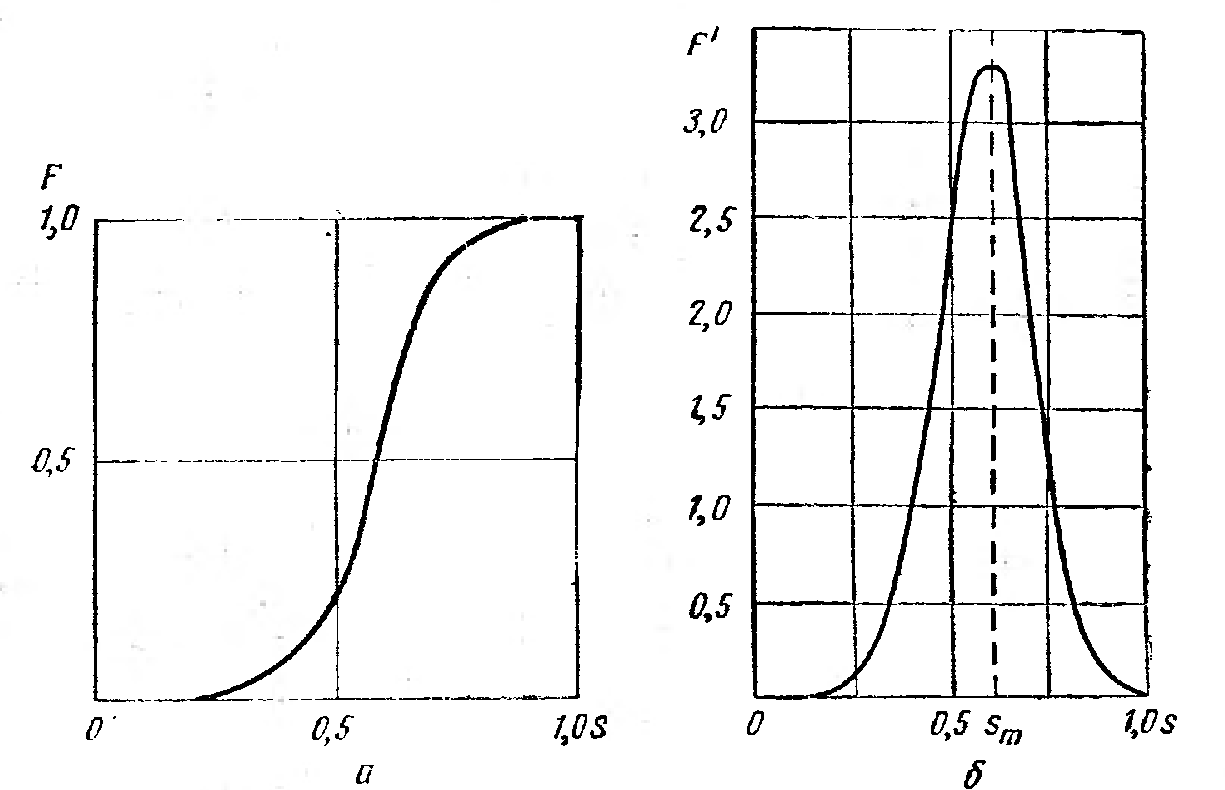
\includegraphics[width=.85\linewidth]{figures/fig-VI-7.png}\caption{}\label{q11:fig-VI-7}\end{figure}
С ростом $Q$ начальное гладкое распределение насыщенности деформируется, как это видно на рис. \ref{q11:fig-VI-8}. В некоторый момент (т. е. при некотором $Q$) касательная к кривой $s(W)$ становится вертикальной. Начиная с этого момента, возникает и распространяется скачок насыщенности. Положение скачков насыщенности заранее неизвестно и должно быть найдено в зависимости от времени из решения задачи. На скачках (поверхностях разрыва) должны выполняться условия непрерывности давления и сохранения массы каждой из движущихся фаз.

Выведем условия на скачках для общего случая неодномерного двухфазного течения. Первое из этих условий записывается в виде:
\begin{equation}p^{(1)}=p^{(2)}.\tag{VI.2.19}\label{q11:eq-VI-2-19}\end{equation}
Рассмотрим теперь условия сохранения массы каждой из фаз при прохождении поверхности разрыва (скачка) через некоторый элемент объема пористой среды (рис. \ref{q11:fig-VI-9}), вырезанный по нормали к поверхности разрыва. В силу непрерывности давления сжимаемость
% Источник: Barenblatt-et-al-1972.djvu; печатная страница: 162; страница файла: 164
жидкостей для условий на скачке несущественна. Применим к этому элементу уравнение сохранения массы \eqref{q11:eq-VI-2-3}. Имеем
\[\frac{d}{dt}\left(\int_Tms\,d\tau\right)=mV_n(s^{(1)}-s^{(2)})A+o(T),\]
где $A$ --- площадь поперечного сечения элемента (индексом 1 сверху обозначены величины за скачком, индексом 2 --- перед скачком); $V_n$ --- скорость перемещения скачка по нормали к нему; $o(T)$ --- величина, стремящаяся к нулю быстрее, чем $T$.
\begin{figure}[H]\centering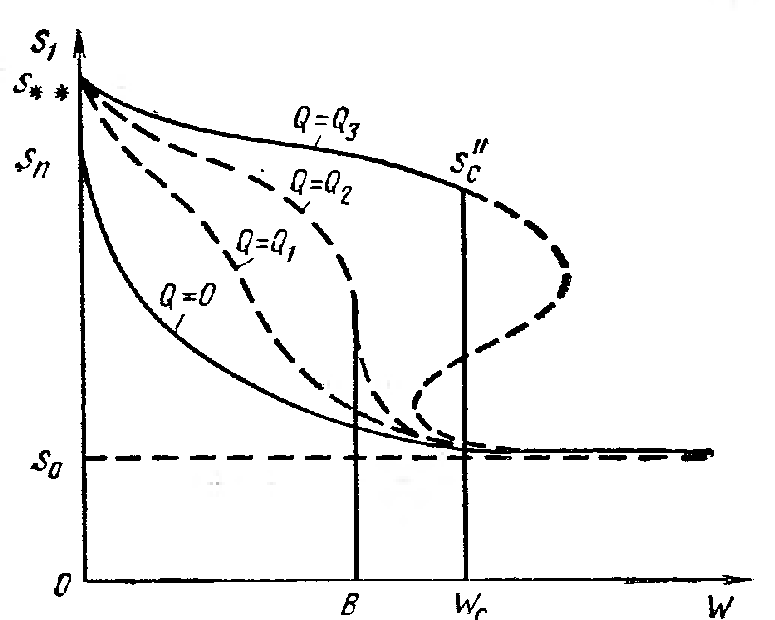
\includegraphics[width=.65\linewidth]{figures/fig-VI-8.png}\caption{}\label{q11:fig-VI-8}\end{figure}
\begin{figure}[H]\centering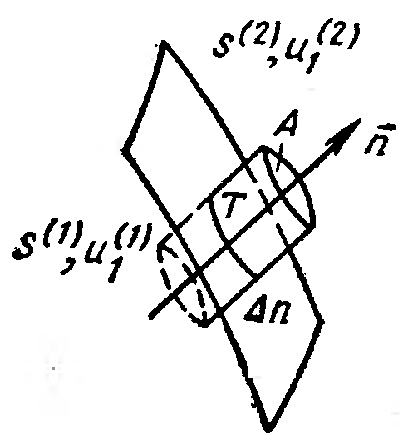
\includegraphics[width=.4\linewidth]{figures/fig-VI-9.png}\caption{}\label{q11:fig-VI-9}\end{figure}
Поток жидкости через сечения, параллельные поверхности разрыва, равен $(u_{1n}^{(1)}-u_{1n}^{(2)})A$ ($u_{1n}$ --- проекция скорости фильтрации первой фазы на нормаль к поверхности скачка). Поток, связанный с касательной составляющей скорости, исчезающе мал по сравнению с $u_{1n}A$ при стремлении $\Delta n$ к нулю в силу условия \eqref{q11:eq-VI-2-19}.

Условие сохранения массы первой жидкости примет тогда вид:
\begin{equation}mV_n(s^{(1)}-s^{(2)})=u_{1n}^{(1)}-u_{1n}^{(2)}.\tag{VI.2.20}\label{q11:eq-VI-2-20}\end{equation}
Равенство \eqref{q11:eq-VI-2-20} можно переписать в виде:
\begin{equation}V_n=\frac{u_{1n}^{(1)}-u_{1n}^{(2)}}{m(s^{(1)}-s^{(2)})}.\tag{VI.2.21}\label{q11:eq-VI-2-21}\end{equation}
Условие сохранения массы второй жидкости также сводится к выражению \eqref{q11:eq-VI-2-20}, поскольку
\begin{equation}u_{1n}^{(1)}+u_{2n}^{(1)}=u_{1n}^{(2)}+u_{2n}^{(2)}.\tag{VI.2.22}\label{q11:eq-VI-2-22}\end{equation}
Вернемся к исследуемой одномерной задаче. Из определения функции $q(t)$ и $F(s)$ можно записать выражения для скоростей фильтрации вытесняющей фазы позади и впереди скачка:
\begin{equation}u_1^{(i)}=\frac{q(t)}{x^\nu}F(s^i)\qquad(i=1,2),\tag{VI.2.23}\label{q11:eq-VI-2-23}\end{equation}
% В (VI.2.23) напечатан показатель ν, а в (VI.2.24) — ν−1; сохранено.
% Источник: Barenblatt-et-al-1972.djvu; печатная страница: 163; страница файла: 165
где индекс 1 относится к величинам за скачком, индекс 2 --- перед скачком. Тогда получим следующее выражение для скорости скачка $V_n=V=dx/dt$:
\begin{equation}\frac{dx}{dt}=\frac{q(t)}{mx^{\nu-1}}\frac{F(s^{(1)})-F(s^{(2)})}{s^{(1)}-s^{(2)}}.\tag{VI.2.24}\label{q11:eq-VI-2-24}\end{equation}
Переходя к переменным $W$ и $Q$, получим
\begin{equation}\frac{dW}{dQ}=\frac{F(s^{(1)})-F(s^{(2)})}{s^{(1)}-s^{(2)}}.\tag{VI.2.25}\label{q11:eq-VI-2-25}\end{equation}
Распределение насыщенности по обе стороны скачка описывается формулой \eqref{q11:eq-VI-2-15}. Положение скачка $W_c$ и насыщенность на скачке $s_c=s^{(1)}$ можно определить вычислением последовательными шагами, исходя из начального положения скачка (т. е. места появления вертикальной касательной), по формуле \eqref{q11:eq-VI-2-25}.

Выведем дифференциальное уравнение, описывающее изменение насыщенности на скачке в зависимости от $Q$. Для насыщенности на скачке, как и для любого значения насыщенности, выполняется соотношение \eqref{q11:eq-VI-2-15}:
\begin{equation}W_c=QF'(s_c)+W_0(s_c).\tag{VI.2.26}\label{q11:eq-VI-2-26}\end{equation}
Очевидно, согласно \eqref{q11:eq-VI-2-26}, $s_c=s^{(1)}$ меняется с изменением $Q$ (т. е. со временем). Дифференцируя \eqref{q11:eq-VI-2-26} по $Q$, имеем
\begin{equation}\frac{dW_c}{dQ}=F'(s_c)+[F''(s_c)Q+W'_0(s_c)]\frac{ds_c}{dQ}.\tag{VI.2.27}\label{q11:eq-VI-2-27}\end{equation}
Приравнивая выражения для скорости распространения скачка насыщенности \eqref{q11:eq-VI-2-25} и \eqref{q11:eq-VI-2-27}, придем к следующему уравнению для $s_c$:
\begin{equation}\frac{ds_c}{dQ}=\frac{F(s_c)-F(s^{(2)})-F'(s_c)(s_c-s^{(2)})}{(s_c-s^{(2)})[F''(s_c)Q+W'_c(s_c)]}.\tag{VI.2.28}\label{q11:eq-VI-2-28}\end{equation}
% В знаменателе оригинала W'_c(s_c), тогда как в (VI.2.27) W'_0(s_c); сохранено.
Значение $s^{(2)}$ в уравнении \eqref{q11:eq-VI-2-28} является функцией $Q$ и $s_c$. Оно определяется из условия $W(s^{(2)})=W(s_c)=W_c$ в соответствии с формулой \eqref{q11:eq-VI-2-15}:
\begin{equation}QF'(s_c)+W_0(s_c)=QF'(s^{(2)})+W_0(s^{(2)}).\tag{VI.2.29}\label{q11:eq-VI-2-29}\end{equation}
Для решения уравнения \eqref{q11:eq-VI-2-28} начальные значения $s_c$ и $Q$ определяются в той точке, где $dW/ds$, соответствующее формуле \eqref{q11:eq-VI-2-15}, впервые обращается в нуль.

Из уравнения \eqref{q11:eq-VI-2-28} следует, что на скачке насыщенности, по обе стороны которого $s_c$ и $s_0=s^{(2)}$ постоянны (стационарный скачок), должно выполняться условие
\begin{equation}\frac{F(s_c)-F(s_0)}{s_c-s_0}=F'(s_c).\tag{VI.2.30}\label{q11:eq-VI-2-30}\end{equation}
% Источник: Barenblatt-et-al-1972.djvu; печатная страница: 164; страница файла: 166
Это условие (полученное впервые в работе Баклея и Леверетта [134]) означает, что скорость распространения скачка равна скорости распространения насыщенности на скачке $s_c$.

Рассмотрим отдельно случай, когда начальная насыщенность $s(W,0)=s_0$ постоянна во всем пласте. Тогда $W_0(s)=0$ при $s>s_0$ и $W_0(s)$ неопределено при $s<s_0$. Из формулы \eqref{q11:eq-VI-2-15} имеем в данном случае
\[W=QF'(s)\qquad(s>s_0).\]
Предположим, что $s_0<s_m$ (см. рис. \ref{q11:fig-VI-7}, \textit{б}), и скачок возникает. При заданных условиях в уравнении \eqref{q11:eq-VI-2-28} переменные разделяются.

Обозначим $s_c-s_0=y$, $F(s_c)-F(s_0)=\psi(y)$. Тогда из уравнения \eqref{q11:eq-VI-2-28}, интегрируя, получим
\begin{equation}\psi(y)-y\psi'(y)=\frac{C}{Q};\quad C=\mathrm{const}.\tag{VI.2.31}\label{q11:eq-VI-2-31}\end{equation}
Поскольку при $Q\to0$ (в начальный момент), левая часть равенства \eqref{q11:eq-VI-2-31} остается ограниченной, $C$ должно обращаться в нуль. Следовательно, скачок является стационарным. Возвращаясь к переменным $s_c$ и $s_0$, получаем, что на скачке при любых $Q$ выполняется соотношение \eqref{q11:eq-VI-2-30}.

Пусть начальное распределение насыщенности таково, что $W_0(s)<0$ при всех $s$, а при $W\to\infty$ $s(W,0)\to s_0$. Тогда рассмотренное выше решение для случая $s_0=\mathrm{const}$ будет выполняться асимптотически при $Q\to\infty$, поскольку $W'_0(s_c)$ ограничено.

Рассмотренное решение и условие \eqref{q11:eq-VI-2-30} было получено Баклеем и Левереттом [134]. Исследование движения скачков насыщенности выполнено С. Н. Бузиновым и И. А. Чарным [36].

В общем случае неодномерной задачи системы \eqref{q11:eq-VI-2-7} и \eqref{q11:eq-VI-2-8} даже при $\varepsilon=0$ уже не сводятся к одному уравнению для насыщенности. Необходимо определять $p$ и $s$ совместно. При этом граничные и начальные условия для $p$ те же, что и в задачах фильтрации однородной жидкости.

Условия для $s$ имеют вид \eqref{q11:eq-VI-2-17} или \eqref{q11:eq-VI-2-18}. Кроме того, на скачках, положение которых заранее неизвестно, должны выполняться условия \eqref{q11:eq-VI-2-19}, \eqref{q11:eq-VI-2-22} и \eqref{q11:eq-VI-2-23}. Решения неодномерных задач могут быть получены лишь численно на ЭВМ.

\end{document}
